\label{sec:metodologia}

Para la selección de un conjunto de ubicaciones idóneas para la implementación de las soluciones propuestas se decidió seguir un enfoque de selección 
multi-criterio soportado en operaciones de lógica difusa.  El diagrama \ref{fig:plan} ilustra esquemáticamente los pasos de la metodología propuesta.  Esta 
metodología puede dividirse en tres partes para su explicación.  Primero, un conjunto de capas son preparadas a partir de una serie de indicadores 
socio-económicos y físicos. Luego, dichas capas son transformadas para estandarizar su magnitud y dimensiones.  Finalmente, se asigna un peso a cada capa de 
acuerdo a su importancia y  se aplica una operación de agregación sobre todas las capas para consolidar un único resultado.  A continuación se explica en más 
detalle los pasos seguidos en cada parte de la metodología.

\begin{figure}
    \centering
    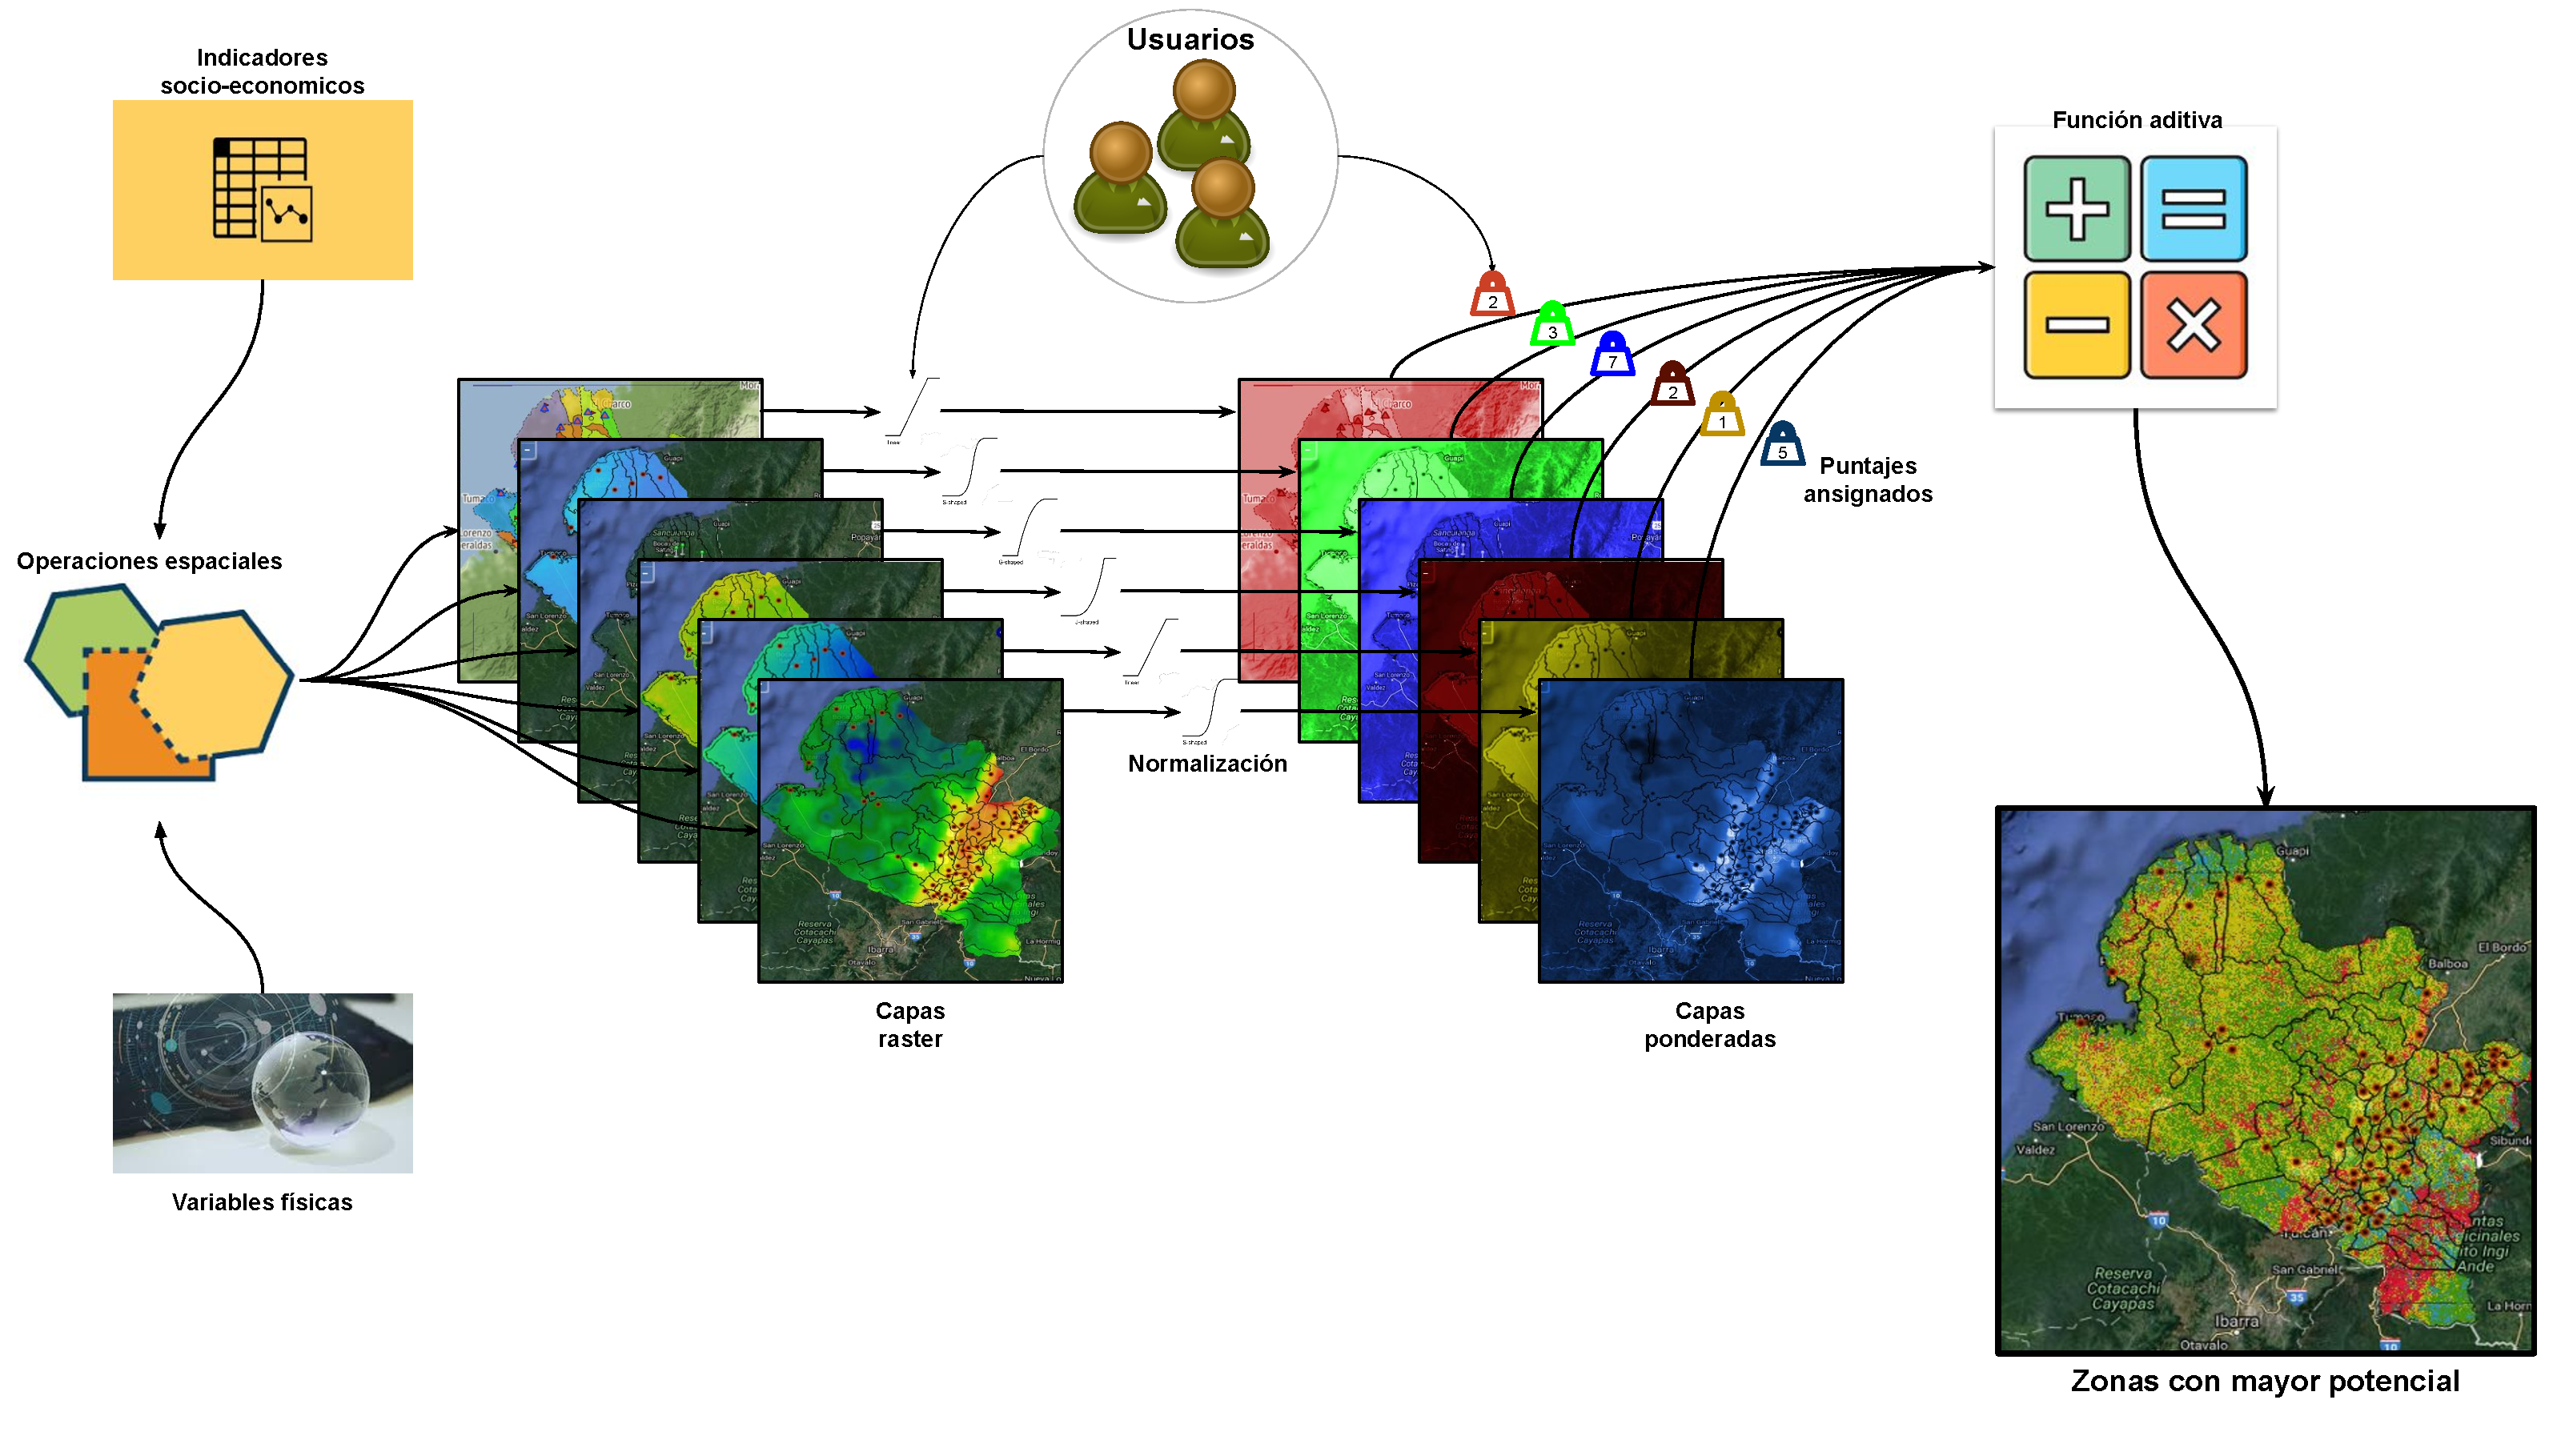
\includegraphics[width=1\textwidth]{figures/plan}
    \caption{Diagrama esquemático de la metodología propuesta.}
    \label{fig:plan}
\end{figure}

En la sección \ref{sec:fuentes} se establecieron las fuentes de datos de los indicadores tenidos en cuenta dentro de esta metodología.  En la primera parte, 
se hizo necesario hacer cierto tratamiento en cada una de ellas.  En particular, todas las capas referentes a indicadores socio-económicos 
se obtuvieron en un esquema tabular, esto es una tabla donde aparece el valor de cada indicador junto con otras variables relacionadas al fenómeno a nivel de 
los municipios de Colombia.  Se tuvo en cuenta el código DANE de cada municipio junto con el valor relacionado a la variable en cuestión.  
Posteriormente, se ejecutó un cruce de datos entre la información extraída y el mapa oficial DANE para georreferenciar los datos y generar una vista de la 
distribución geográfica del indicador.  De esta manera se obtienen una serie de mapas que ilustran la composición del indicador para cada municipio.

Para las variables físicas también se hizo necesario aplicar ciertas operaciones espaciales para ajustar los conjuntos de datos iniciales a las condiciones del 
área de estudio.  Por lo general, para estos casos, los estudios son de carácter global, por lo que se requería extraer los datos solo para el territorio 
Colombiano.  Según el caso, fue necesario aplicar operaciones de agregación espacial, si los datos para Colombia se presentaban en más de una fuente, o 
temporales, si se proveían datos a nivel mensual y lo requerido eran promedios anuales.  Visualizaciones de los mapas obtenidos en esta etapa están disponibles 
como anexos digitales a este informe dentro de la carpeta \textit{mapas}.

Para la segunda parte de la metodología, se requiere que todas las capas se encuentren en una versión raster de idénticas dimensiones (esto es 
una imagen con igual número filas y columnas donde el valor de cada píxel sea el valor del indicador que representa).  En esta etapa, se aplicaron operaciones 
espaciales a las capas de indicadores socio-económicos para convertir su versión vectorial (polígonos representando cada municipio) a capas raster.  Como 
dimensiones específicas se seleccionó un área de 1666 columnas por 1972 filas que cubre la extensión del mapa oficial DANE usando un sistemas de coordenadas 
EPSG:3857 (Pseudo-Mercator).  La resolución espacial obtenida fue de aproximadamente 1 Km$^2$.  Se reprojectaron y se ajustaron todas las capas (incluyendo las 
variables físicas) a dichas dimensiones y al sistema de coordenadas mencionado para permitir su análisis en unidades de metros.

Para permitir la aplicación de una función de agregación todas las capas deben ser tratadas para transformar sus valores y rango de datos a un estándar común.  
La lógica difusa provee una serie de funciones de membresía que permiten escalar los datos de 0 a 1 donde el usuario puede especificar valores a priorizar y 
diversas clases de curvas para transformar los datos.  La membresía lineal es la más sencilla de las funciones y se corresponde a una normalización típica.  
Dadas las características de las capas de entrada se decidió utilizar esta membresía ya que no era necesario la aplicación de funciones más elaboradas. 
Los valores para cada variable se escalan asignando un valor de 0 al valor con menor prioridad y un valor de 1 al más alto, los valores intermedios se obtienen 
a travéz de una interpolación directa.  

En la última parte de la metodología, contamos con una serie de capas raster ponderadas y unificadas.  Cada píxel en las imágenes se corresponde uno a uno por 
lo que cualquier operación de agregación es valida.  La operación de agregación tomará cada píxel de las capas en la misma ubicación y los agregará de acuerdo 
a su función, el resultado será el valor del píxel en dicha ubicación para el mapa final.  De nuevo, la lógica difusa provee diferentes funciones de 
agregación pero dadas las características del estudio se decidió utilizar una sumatoria simple.  Cabe aclarar que previo a la operación de agregación se 
asignaron pesos distintivos a cada capa.  Esto es, un valor por el cual se multiplica el valor de cada píxel antes de operarlo con los demás.  Generalmente, la 
asignación de pesos a cada capa se hace de manera coordinada entre los interesados y expertos y puede ser fácilmente editada en el modelo final para su 
posterior ejecución.  

En la actual implementación, se decidió asignar un puntaje de 3 puntos a 3 capas específicas: la cobertura del servicio de energía eléctrica, con el fin de 
priorizar aquellas zonas con déficit de dicho servicio; el rendimiento agrícola, para priorizar áreas con alta producción de residuos agrícolas que puedan ser 
aprovechados como biomasa; y los casos positivos de COVID-19, con el objeto de beneficiar los municipios más afectados por la pandemia.  Al resto de 
indicadores socio-económicos se le asignó un puntaje de 2 puntos y a todas las variables físicas se les dio un peso de 1 punto.  Se priorizaron las variables 
socio-económicas sobre las físicas por el contexto de la investigación donde se busca resaltar mas los beneficios a poblaciones vulnerables sobre aspectos de 
eficiencia o retorno de la inversión.

El mapa obtenido en esta etapa es finalmente escalado, entre 0 y el máximo valor posible de acuerdo a los pesos asignados, obteniendo una capa raster con 
valores entre 0 y 1 para cada ubicación en el mapa a manera de un índice.  Para obtener un indicador a nivel de municipio, se utiliza una capa adicional para 
agregar por zonas y calcular el promedio de todos los píxeles contenidos en un respectivo municipio.  Esto entrega una capa vectorial, con cada municipio 
relacionado con su valor promedio de acuerdo al puntaje obtenido en el índice anterior.  Esta lista de municipios y su valor promedio se utiliza como una 
clasificación para la selección de los municipios con mayor potencial para la implementación de las soluciones propuestas en las posteriores etapas de la 
investigación.
